\documentclass[senior]{IPSstyle}


\Year{2020}
\Month{July}
\Author{44181528-1}

\Title{DualBox}

\Advisor{Professor YOSHIE}

\usepackage{amssymb,amsmath}

\usepackage{array}
\usepackage{mathptmx}
\usepackage{helvet}
\usepackage{courier}
\usepackage{type1cm}

\usepackage{makeidx}
\usepackage{graphicx,subfigure}
\usepackage{multicol}
\usepackage{multirow}
\usepackage[bottom]{footmisc}

\usepackage{mathrsfs}
\usepackage{amssymb,amsmath}
\usepackage{amsfonts}
\usepackage{color}
\usepackage{CJKutf8}
\usepackage{smartdiagram}
\usepackage{caption}

\usepackage{listings}
\usepackage{algorithm,algorithmicx,algpseudocode}
\usepackage[toc,page,title,titletoc,header]{appendix}

\DeclareMathOperator*{\otherwise}{otherwise}

\renewcommand{\algorithmicrequire}{\textbf{Input:}}
\renewcommand{\algorithmicensure}{\textbf{Output:}}

\Abstract{Consensus building process for enterprise digital transformation is a significant approach on the implementation of Internet of Things (IoT) solutions through product lifecycle management (PLM). When we improve the consensus building process, it is important to find any latent opinions and hidden dialog patterns analyzing discussion activities by stakeholders. Several approaches have been proposed in forms of instructions and frameworks such as causal model of Consensus Building Theory (CBT) and short-term intensive workshop in strategy planning phase of Product Lifecycle Management (PLM) process. This paper will analyze a new approach to improve consensus building process by summarizing discussion activity. The proposed method is done by performing data augmentation and topic modeling with the help of background knowledge on discussion activity held within industrial engineering context. Our method produces a complete summarization of discussion activity that consists of topic distribution and distribution similarity between topics. We also found that the usage of data augmentation and background knowledge will improve topic quality. We validate our findings to a professional consultant and conclude that our approach gives an adequate contribution towards summarizing discussion activity that might improve consensus building process.}

\Keywords{Topic Model, Background Knowledge, Consensus Building, Product Lifecycle Management, Data Augmentation}

\Acknowledgments{Completing master’s degree is a great and valuable experience for me. Studying abroad gave me a lot of interesting knowledge to take advantage of. I would like to thank Prof. Yoshie and Goto-san who have guided me throughout my master’s thesis. I also would like to thank Rococo, ltd. as my main financial support and the organization that enables me to study in Japan. All The knowledge I retrieved is very important for my next journey and my career. 

During my time I spent in Kitakyushu, I got a lot of love and support from people around me. In this part of the Thesis I would like to thank each one of them. Thanks to my parents and family for taking care of me and letting me choose this path of journey. Thanks to the one and only Miranda that keep supporting and encouraging me during my final months in Kitakyushu. Thank you to my fellow school-mates; Hayden, Palm, and many others from Waseda who stay with me through thick and thin. And finally, thanks to the whole family of PPI Kitakyushu (Indonesian student association in Kitakyushu) that always made me feel like home.}

\begin{document}
\makepreliminarypages
\singlespace
\frontmatter
\tableofcontents
\listoffigures
\listoftables
\mainmatter
\clearemptydoublepage
\setlength{\baselineskip}{23.0pt}

%%%%%%%%%%%%%%%%%%%%%%%%%%%%%%%%%%%%%%%%%%%%%%%%%%%%%%%%%%%%%%Chapter 1
\chapter{Introduction} 
%%%%%%%%%%%%%%%%%%%%%%%%%%%%%%%%%%%%%%%%%%%%%%%%%%%%%%%%%%%%%%Chapter 1

%--------------------------------------------------------------------------
\section{Background and Motivation}
%--------------------------------------------------------------------------

A conventional discussion activity happened when a group of people let out their own opinion with appropriate feedbacks from the other. In industries, discussions are being held in various departments to solve specific problems. We can characterize such discussions as a group of people who shares a same interest aimed to build one single consensus.

Some important features of consensus building process are recording, facilitation, and mediation [1]. Recording in this term stands for creating a physical record of what subject being discussed. Recording can be implemented by recording the whole discussion as a video file or even as simple as taking notes on participant’s utterance. Facilitation in a second hand, help participants work together by providing artefact containing the discussion progress which everyone agrees on. Finally, mediation acts to help opposite parties deal with disagreement. In order to perform mediation, one independent person is needed to resolve disputes with his/her objective point of view.

Consensus building plays a significant role in strategy planning phase of Product Lifecyle Management (PLM) process [2]. Strategy planning phase is involving people from various levels and departments in an organization [1], thus justifies the needs of consensus building approach. The practice of consensus building often still have frequent problems. During discussion activities, various stakeholders with different personalities and backgrounds might influence conclusion [3] which will affect tendency and direction of the discussion [4].

PLM practice also supports manufacturing companies towards digital transformation [5]. As one of the implementations of Internet of Things (IoT) solutions, PLM with its holistic paradigm helped companies to change their internal resources e.g. business processes, product data, and people by taking the benefits of its external resource generated by other IoT solutions. In this research, we propose a better consensus building approach for PLM process which will leads to the advancement of digital transformation

%--------------------------------------------------------------------------
\section{Related works}
%--------------------------------------------------------------------------

Researches related to consensus building have been conducted years ago. In general, researches focused on consensus building can be divided into 2 categories based on their focus point; process model and measurement model. All models are designed under the same goal: to improve consensus quality.

Process model focused on a set of rules that participants should follow under specific circumstances. A research proposed a straightforward approach using a fair, open, and freedom-focused process model [8], meaning that all perspective will be considered equal and all participants will have their freedom to disagree. Another research is focused specifically on a subprocess in consensus building like Consensus Building Theory (CBT) [9] which emphasizes the cause of conflict to investigate what specific matter prevent or support consensus building. Other research is focused on a specific implementation of process model [4] e.g. proposing a short term and intensive workshop activity designed for Product Lifecycle Management (PLM) strategy planning phase which involves multi-party stakeholders. The workshop is intended specifically for discussion under digital transformation for smart, connected engineering field.

Meanwhile, measurement model focused more on the criteria to determine consensus presence. Some popular methods are done by using standard deviation of voting results or using Kendall’s coefficient on voting results [10]. A recent method showed that a digitized approach can be done by tracking every non-verbal aspects of each participant to determine consensus [7]. Another digitized approach has been done in 2 steps: inviting external facilitator as one independent figure to direct the course of discussion and doing text mining approach on the dialog data taken from the discussion to evaluate consensus [6].

%--------------------------------------------------------------------------
\section{Research Problem}
%--------------------------------------------------------------------------

Previous researches discussed on how consensus is being built by considering a lot of variables e.g. time consumed, participants contributions, and conflict resolution method. In another hand, more variables should be valued more such as the objectivity of the final consensus and the latent opinion from each participant. A preliminary study regarding this matter has been conducted [6] but it risks of having biased judgment which will damage consensus building process. We proposed a better text mining approach by utilizing topic model algorithms, a set of data as Background Knowledge, and calculating the convergence rate among topic distributions. Data augmentation is also added in the process to increase data quality.

%--------------------------------------------------------------------------
\section{Organization of Thesis}
%--------------------------------------------------------------------------

In this chapter, we discussed about fundamental knowledge of consensus building and PLM, we explained previous works related to consensus building, and we discussed about the undiscovered aspects on how to improve consensus building process as our hypothesis. Chapter II will explain the proposed methodology we used to perform a digitized text mining approach to improve consensus building process. In chapter III, we conduct the experiment to figure out the best topic model configuration to be used. Chapter IV is the implementation and validation of our findings by quantitative evaluation and qualitative review. Finally, in chapter V, we will summarize what we have achieved so far and provide future research directions.

%%%%%%%%%%%%%%%%%%%%%%%%%%%%%%%%%%%%%%%%%%%%%%%%%%%%%%%%%%%%%%Chapter 2
\chapter{Proposed Method} 
%%%%%%%%%%%%%%%%%%%%%%%%%%%%%%%%%%%%%%%%%%%%%%%%%%%%%%%%%%%%%%Chapter 2

In this research, we performed a digitized approach of dialog data from PLM-themed discussion activity sessions using data augmentation, topic model with background knowledge, and distribution similarity. First, the data will be prepared by a simple preprocess method and data augmentation. The clean and augmented data will then be experimented by various topic models and hyperparameters, we picked the best configuration and incorporate it into background-knowledge-backed topic model to generate topic distributions. Then, we will calculate the distribution similarity as convergence rate. Finally, we will compare the effectiveness of our approach to previous research and get a professional consultant to analyze the topic distribution results to have an objective review. To summarize, we will take dialog data of discussion session and transform it into topic distributions, similarity value, and most frequent words (if necessary) from each discussion session to be validated by a professional consultant.

%--------------------------------------------------------------------------
\section{Data Augmentation}
%--------------------------------------------------------------------------

We took a real-life dialog data from discussion sessions which ran for 1-2 hour long. Based on the dataset characteristics in Table 1, the dataset we used is very poor. Compared to the common dataset in topic model research with specialization in short text data, our dataset size is 96.55\% lower in terms of number of documents and 85.96\% lower in terms of corpus size. Hence, we are using data augmentation techniques to improve dataset quality. We expand the Easy Data Augmentation [12] by adding additional processes: hypernym replacement and hyponym replacement. Hypernym and hyponym of a word is crucial as we thought the topic mixture of a sentence \textit{s} should be the same with another sentence \textit{s’} who has hypernym/hyponym relation with it.

The augmentation process will produce additional sentences that is similar sentence for what it refers to. For example, sentence ‘john eat apple’ will produce at least 2 sentences: ‘john eat apple’ (original sentence) and ‘john consume apple’ (augmented sentence by replacement). If our dataset is having 100 sentences, it will produce at least 200 sentences as a new dataset.

%--------------------------------------------------------------------------
\section{Topic Model with Background Knowledge}
%--------------------------------------------------------------------------

We tried to mine latent opinion of the dataset using topic model with background knowledge. Topic model is an unsupervised learning approach where we could transform documents into document-to-topic distributions and topic-to-word distributions. In topic model point of view, document is a mixture of topic where topic itself is a mixture of word. The most popular method of topic model is Latent Dirichlet Allocation (LDA) [13], in which, current topic model researches mostly use LDA as baseline method. In LDA-based topic model, the learning process consists of generation process and sampling process. In generative process, the initial document-to-topic distributions and topic-to-word distributions are generated using hyperparameter ALPHA and BETA. Then, in the sampling process, distributions are evaluated by recalculating it using Gibbs Sampling for each word. The graphical notation of LDA topic model is shown in Fig. 1. Meanwhile, the generation algorithm is shown in Fig. 2 where K is number of topics, D is number of documents, Nd is number of words in document d, PHI k is topic-to-word distribution for topic k, THETA d is document-to-topic distribution for document d, z id is topic for the i th word in document d, and w id is the i th word in document d.

We mentioned in previous paragraph that our dataset has relatively smaller size compared to common topic model researches. Hence, we assembled various topic models with specialty in short text as suggested by [11]. The whole list of topic models could be seen in Table 2 that could be categorized into 4 types. The first type is standard, referred to the baseline topic model which is LDA. The second type, one-topic sampling based, will modify the inference process to sample only one topic per document, meaning all words from a single document will only have one topic label. The third type, global word co-occurrence based, will modify document representation into word-network or set of biterms. Self-aggregation based as the last type will merge several documents into one single pseudo-document and then apply standard-type topic model to it.

After the experiment is done, we will decide what is the best topic model, hyperparameters, and the number of sentence augmentation processes to use. After that, we will incorporate the result to a new background-knowledge-backed topic model called Source-LDA [14] as the most suitable topic model for our case. In Source-LDA, we can use background knowledge data to influence topic labeling thus improving topic
quality in the process.

%--------------------------------------------------------------------------
\subsection{Dirichlet Multinomial Mixture [16]}
%--------------------------------------------------------------------------

The main feature of this topic model is by assuming that each document is sampled by only one topic. Thus, assuming all the words from corpus is sampled under a single multinomial distribution ( THETA ). This assumption is proven to be effective in some cases and a lot of other topic model is proposed based on this assumption.

%--------------------------------------------------------------------------
\subsection{Latent-Feature LDA [17]}
%--------------------------------------------------------------------------

This topic model doesn’t explicitly belong to ‘one-topic assumption’ category. However, this topic model is proposed together with ‘Latent-feature DMM’ so we put it under the same category for the sake of simplicity. The main feature of this topic model is by using external word vectors to perform a better inference on topic of each words. The inference is done by sampling a binary indicator variable from Bernoulli distribution to pick a new topic from Dirichlet distribution or latent feature vector.

%--------------------------------------------------------------------------
\subsection{Latent-Feature DMM [17]}
%--------------------------------------------------------------------------

This topic model is using the same method as ‘Latent-Feature LDA’. However, this is based on ‘one-topic assumption’ so it is only using a single Dirichlet distribution ( THETA ) to
infer topic of each words.

%--------------------------------------------------------------------------
\subsection{Generalized Polya Urn DMM [18]}
%--------------------------------------------------------------------------

This topic model uses Generalized Polya Urn (GPU) model to improve topic inference. The GPU model itself is described as follow: for every colored ball picked up from a jar, a couple more balls from the same color will be returned. In this case, this topic model will increase the probability of topic k of words that has close meaning with word w using ‘Promotion Matrix’. The rest of the methods of this topic model is the same with DMM.

%--------------------------------------------------------------------------
\subsection{GPU Poisson-based DMM [19]}
%--------------------------------------------------------------------------

The main feature of GPU-PDMM is using Poisson distribution to determine the number of topics that can generate a single document d that is limited by specific threshold. The topics of each document is written as Z d , the mean value of Poisson distribution is LAMBDA, and the t d is the number of topics that generate document d.

%--------------------------------------------------------------------------
\subsection{Biterm Topic Model [20]}
%--------------------------------------------------------------------------

BTM deals with word representation in each document. Instead of single word, BTM treats each document as a collection of biterms where each neighboring word are counted as single biterm ( w 1 , w 2 ). Furthermore, topic inference is done for each biterm meaning that each word will be sampled up to 2 times since each word could have been included in 2 biterms.

%--------------------------------------------------------------------------
\subsection{Word Network Topic Model [21]}
%--------------------------------------------------------------------------

Unlike BTM, WNTM will change the document representation instead of word. A sliding window will be applied to collect the co-occurrence of word w . Then, a word network will be created with words as vertices and edge between vertices is the co-occurrence frequency of 2 words ( w i , w j ). Pseudo-document p will be created for each vertex taking every adjacent word as the content.

%--------------------------------------------------------------------------
\subsection{Self-aggregate Topic Model [22]}
%--------------------------------------------------------------------------

SATM assumes that each document d is a short-text snippet sampled from a longer document D . With this assumption, the generation process is slightly modified to form PHI (probability of words in long document D) while also forming phi and theta like standard topic model. Moreover, the inference process also altered to estimate the new topic z and new long document D for each word w.

%--------------------------------------------------------------------------
\subsection{Pseudo-based Topic Model [23]}
%--------------------------------------------------------------------------

PTM assumes that each short text is a snippet sampled from one long document p l. Different with SATM, PTM generates PHI as a multinomial distribution for long documents in a single phase using hyperparameter LAMBDA. Thus, reducing the complexity of the overall algorithm. PHI is again re-estimated in each iteration.

%--------------------------------------------------------------------------
\subsection{Source-LDA [14]}
%--------------------------------------------------------------------------

The main feature of Source-LDA is adding another probability distribution of words for each background knowledge topics. Topic in each word is inferred from both standard topic feature vector PHIk and background knowledge topic feature vector PHIm.

%--------------------------------------------------------------------------
\section{Distribution Similarity}
%--------------------------------------------------------------------------

In this step, we aimed to picture the topic distribution into a single value that describes the rate of consensus built (convergence rate). In order to do this, we used distribution similarity calculation using Jensen-Shannon Divergence across all distributions [15]. This concludes the final step of our proposed method.

%%%%%%%%%%%%%%%%%%%%%%%%%%%%%%%%%%%%%%%%%%%%%%%%%%%%%%%%%%%%%%Chapter 3
\chapter{Experiment} 
%%%%%%%%%%%%%%%%%%%%%%%%%%%%%%%%%%%%%%%%%%%%%%%%%%%%%%%%%%%%%%Chapter 3

In this chapter, we will describe how the experiment process is done. We conducted 4 steps of experiment consists of Preprocessing, Experiment using Standard Topic Model, Experiment using background knowledge Topic Model, and Implementation (will be explained in the next chapter). In the first step, we are focusing on how to prepare the data by doing preprocessing and augmentation process. Experiment using topic models focused on testing combinations of augmentation process, type of topic model, and hyperparameters by looking at their topic coherence value. Finally, implementation step focused on presenting our method by topic distributions and convergence value.

%--------------------------------------------------------------------------
\section{Preprocessing and Augmentation}
%--------------------------------------------------------------------------

We had an opportunity to utilize dialog data from requirement decisions (discussion session) of 4 Japanese companies. Firstly, data preprocessing and sentence augmentation is done to clean the data. The comparison of dataset characteristics before and after augmentation is shown in Table 3. We managed to expand the dataset up to 1634.46\% from the original size in terms of number of documents, and up to 145.04\% in terms of corpus size.

Furthermore, the dataset property is presented in Table 4. During dialog data collecting process, 2 types of question were asked. Problem-type question was given at the early stage of discussion while solution-type question is asked at the later stage of discussion. Another property is ’response category’ that referred to participant’s own division, and ’organization level’ that referred to participant’s hierarchical level in the company.

%--------------------------------------------------------------------------
\section{Experiment using Standard Topic Model}
%--------------------------------------------------------------------------

Following data preprocessing step, topic model experiment is conducted on all topic models in Table 2. We used topic coherence value to evaluate topic model performance because our dataset is raw and doesn’t have any golden labels [11]. The result of topic model experiment is shown in Fig. 6. The hyperparameter used in this experiment is number of iteration (1000-2000), ALPHA value (0.05-0.3), and BETA value (0.005-0.03). The number shown in the figure is the average of topic coherence value of all possible hyperparameters for each sentence augmentation processes. Based on the number of sentence augmentation, 9 augmentation is not producing significant result while 1 augmentation gives the best and most consistent result. Self-Augment Topic Model (SATM) gives a good overall score regardless the number of sentence augmentation process. However, LDA held the best score of all experiment with 1 augmentation process. We picked LDA topic model with ALPHA value of 0.15, BETA value of 0.01, 2000 iteration, and 1 sentence augmentation process as the best configuration.

%--------------------------------------------------------------------------
\section{Experiment using Topic Model with Background Knowledge}
%--------------------------------------------------------------------------

The next step is to incorporate the best configuration into Source-LDA. Because Source-LDA is based on LDA, we only modified the hyperparameters during this experiment. Based on our proposed method in Section II, we are using PLM-themed discussion activity as our dataset. Hence, PLM topics is used as the background knowledge data. We decided to use PTC Value Roadmap 1 because it contains many PLM Topics with complete definitions for each topic. The background knowledge dataset held a relatively big size consisting of 26 topics, 1068 unique words, and 145.88 average document length.

Fig. 7 shows the topic coherence value relative to the number of sentence augmentation process applied to background knowledge dataset. The topic coherence value is increasing proportionally with the number of sentence augmentation. The usage of sentence augmentation on background knowledge improves topic coherence up to 3.25\%. We picked 12 sentence augmentation process on background knowledge as the best configuration.

The final best configuration we found is by using LDA topic model, ALPHA value of 0.15, BETA value of 0.01, 2000 iteration, 1 sentence augmentation on dialog dataset, and 12 sentence augmentation on background knowledge. We are planning to use this finding in future experiment.

%%%%%%%%%%%%%%%%%%%%%%%%%%%%%%%%%%%%%%%%%%%%%%%%%%%%%%%%%%%%%%Chapter 4
\chapter{Results and Discussion} 
%%%%%%%%%%%%%%%%%%%%%%%%%%%%%%%%%%%%%%%%%%%%%%%%%%%%%%%%%%%%%%Chapter 4

This chapter will explain ‘implementation step’ as described in previous paragraph. First, we will quantitatively compare the quality of topic distributions generated using our recommended configuration to previous research [6]. Then, we will ask a professional consultant to do qualitative evaluation towards our result.

%--------------------------------------------------------------------------
\section{Quantitative Evaluation: Topic Coherence Value}
%--------------------------------------------------------------------------

We compared our findings with previous research [6] as shown in Fig. 8. We compared between both approaches using topic coherence value. We improved the result by 6.34\% by utilizing data augmentation and background knowledge.

%--------------------------------------------------------------------------
\section{Qualitative Evaluation: Review by Professional Consultant}
%--------------------------------------------------------------------------

We implemented our model to create topic distributions of the dataset. Then, we calculate the convergence rate among topic distributions and do qualitative evaluation together with external facilitator.

During topic modeling process, we replaced background knowledge’s topic name with its topic number to increase readability. The mapping of topic number with its actual name can be seen at Table 5 with a side note that the order of topic number is in alphabetical order and different with what shown in the reference (PTC Value Roadmap). There are 26 PLM Topics in total that serves as best practice for a specific business unit.

The average topic distribution of sentences in dialog data from each company is shown in Fig. 9. The most probable and least probable topic is different for each company. For example, company 1 that runs in business process innovation industry discussed a lot about topic \#12 (Project Management) and very little about topic \#24 (Verification and Validation). Meanwhile, Company 2 from automotive manufacturer industry had a huge interest in topic \#18 (Service Order Management and Field Service) but not in topic \#22 (Technical and Service Parts Information Creation and Delivery). Company 3 from aqua industry has topic \#19 (Service Parts Planning and Pricing) as the most probable topic and topic \#2 (Component and Supplier Management) as the least probable topic. Lastly, company 4 from automotive supplier industry had topic \#22 and topic \#21 (System Architecture Design) as their most probable topics.

Given the topic distributions, we will conduct similarity measurement using JS Divergence to find convergence rate. The interpretation value of JS divergence ranges from 0-1. All value approaching to 0 means that there is no variation between probability distributions, meanwhile value approaching to 1 means that there is high variation between probability distributions. The convergence of each discussion sessions can be seen at Table 6 along with the top frequent words. The overall convergence rate achieved from each discussion is probably not too good since each one has convergence rate above 0.500. The lowest degree of convergence was achieved by Company 1 with 0.865 while the highest degree of convergence was achieved by Company 3 with 0.672. The top words from each discussion acts as a support to better understand the discussion.

Given the results, here is the feedback from professional consultant for each discussion session:

\paragraph{Company 1} Company 1 had a key problem in terms of information exchange between design and manufacturing. I agree that the frequency of Design and Manufacturing topics was high. However, the topic of Project Management was rarely spoken directly by their voices. In addition, the analysis results show that there are few topics on Manufacturing Process Management. Certainly, there were few remarks on Manufacturing Process Management when the workshop was held. However, one of the participants was very concerned about the topic and he is one of the important people in the PLM project, so even if it is a minority opinion, I cannot ignore it as my consultant perspective. By the way, in the analysis results, the words with the highest frequency of occurrence were Information, Product, and Data. These were key words that participants often talked about during the actual workshop. As a consultant, I agree with that.

\paragraph{Company 2} The company 2 had three business unit. Thus, the participants had different opinions, as each business unit had a completely different product and each business model was different. When I looked at the results of this analysis, I thought that the reason that the topic of Verification and Validation was high was probably that they had a problem with their product quality. However, although the topic about Field Service has not been talked about in the actual workshop time, the frequency of topic 18 was high in this analysis result. In fact, this company does little field service work, so it is necessary to confirm why such analysis results were performed. In addition, the analysis results indicated that the frequency of Product Cost Management and Project Management topics was low. However, I think the discussions about costs and projects were relatively common during the actual discussions with them. Regarding the word distribution, the analysis result, it showed that the frequency of Production, Work, and Product were high. I agree with this result.

\paragraph{Company 3} The motivation for Company 3 to introduce PLM was to strengthen its field service operations. Looking at the analysis results, it was found that the topics with the highest frequency were field services, such as Warranty management, Performance Based Contract Management, Technical Service Parts Information, and Service Order Management. I agree this result as a professional consultant. However, regarding the monitoring and management of equipment, it was analyzed that the topic frequency was low. This is different from the actual situation, because in the actual workshop, the story of equipment monitoring was relatively well discussed. The frequency of words of Resource, Human, Product, and Development is high. Even during the actual workshop discussion, the shortage of human resources in field service was very problematic. Thus, I agree with the analysis results.

Company 4: Company 4 has been practicing efforts to make its factory a smart factory. As a consultant, what I noticed in their actual workshops was their lack of information sharing between departments and insufficient training of employees. On the other hand, looking at the results of this analysis, we found that the topic \# 22 was Technical and Service Part Information Creation and Delivery. At first, I wasn’t interested in topic \# 22. However, after reviewing the content of discussions with the workshop participants later, there was an opinion that attention was paid to the management of service parts in order to contribute to sustainable sales. It seems that the results of this analysis have taught me a topic that I did not notice at first. Looking at the analysis results of the word distribution, it seems that three words, Information, Data, and Sharing, appear frequently. This was exactly the issue that was being talked about at the workshop. Additionally, the analysis results seem to indicate that there is no relationship between education and system design. Further investigation is needed as I think education topic should be highly related in the workshop.

Based on our analysis and feedback from professional consultant. We feel that our experiment on the usage of topic model with background knowledge in an industrial engineering discussion activity (in this case, PLM-themed) gives an actual contribution towards discussion summarization in which, might improve consensus building process. The important takeaway of this research is that topic modeling with background knowledge will assist professional consultant to understand more towards participant’s latent opinion.

%%%%%%%%%%%%%%%%%%%%%%%%%%%%%%%%%%%%%%%%%%%%%%%%%%%%%%%%%%%%%%Chapter 5
\chapter{Conclusion} 
%%%%%%%%%%%%%%%%%%%%%%%%%%%%%%%%%%%%%%%%%%%%%%%%%%%%%%%%%%%%%%Chapter 5

In this paper, we analyzed a new digitized approach to improve consensus building process in discussion activity held within industrial engineering context (PLM-themed). Our proposed method consists of performing data augmentation, implementing topic model with background knowledge, and calculating the distribution similarity. Finally, we validate the result on professional consultant. We received good feedback which validates our purpose of using a new approach to improve consensus building process. Moreover, we also found that using data augmentation and background knowledge in topic modeling will improve its topic quality.

However, further approach is still necessary based on two perspective: consensus building and topic modeling. From consensus building perspective, we still need to assure the emotional state of discussion participants when dialog data is recorded. Some variables might aspect the quality and consistency of participant’s opinion. Meanwhile from topic modeling perspective, we are planning to expand Source-LDA so it can afford different data representation like BTM and WNTM does.

\begin{figure}[t]
    \begin{center}
    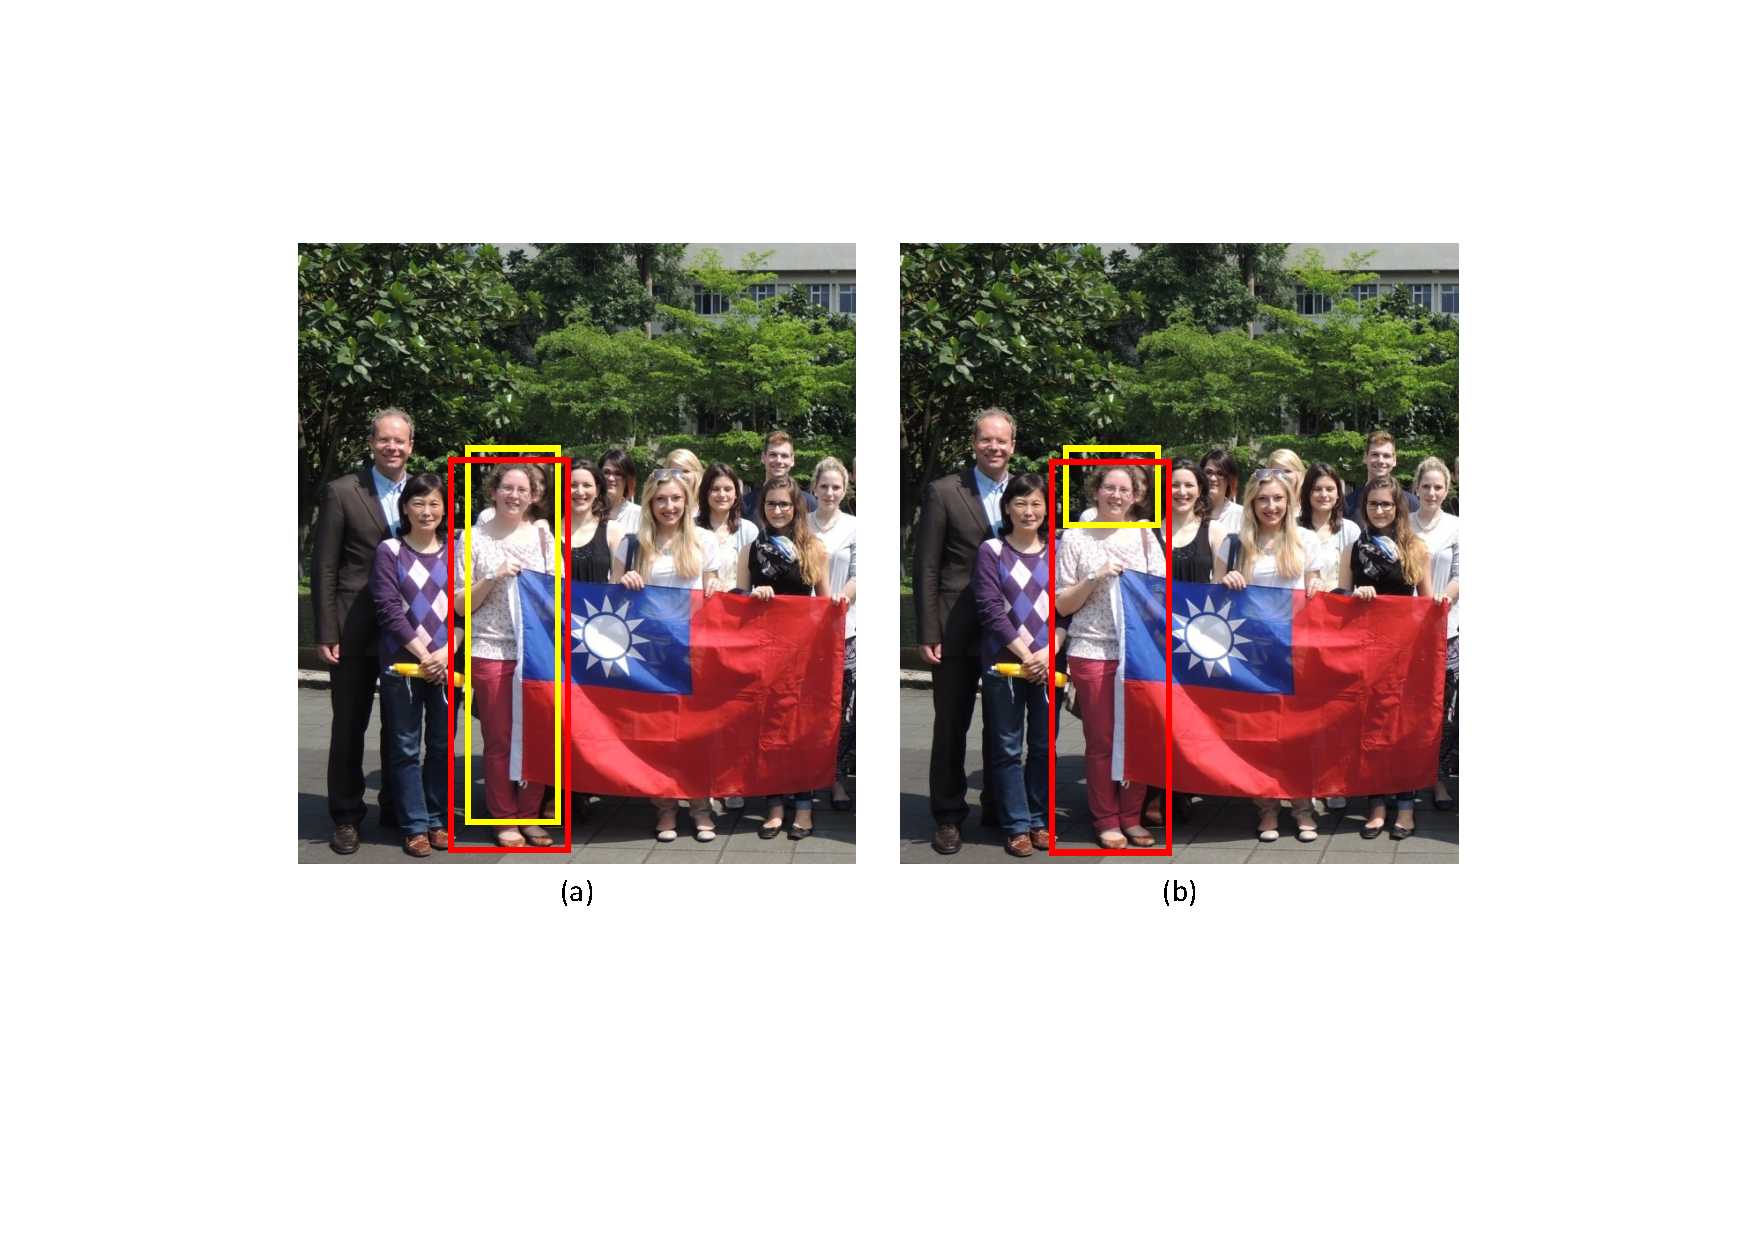
\includegraphics[width=0.97\linewidth]{images/start.pdf}
    \end{center}
\vspace{-0.3cm}
    \caption{ }
    \label{fintro}
    \vspace{-0.3cm}
\end{figure} 


%--------------------------------------------------------------------------
\chapter{References}
%--------------------------------------------------------------------------
\bibliographystyle{plain}
\bibliography{references}

\end{document}